%++++++++++++++++++++++++++++++++++++++++
% Don't modify this section unless you know what you're doing!
\documentclass[letterpaper,12pt]{article}
\usepackage{tabularx} % extra features for tabular environment
\usepackage{amsmath}  % improve math presentation
\usepackage{amssymb}
\usepackage{enumerate}
\usepackage{listings}
\usepackage{graphicx} % takes care of graphic including machinery
\usepackage[margin=1in,letterpaper]{geometry} % decreases margins
\usepackage{cite} % takes care of citations
\usepackage[utf8]{inputenc}
\usepackage{mathtools}
\usepackage[bulgarian]{babel}
\usepackage[final]{hyperref} % adds hyper links inside the generated pdf file
\hypersetup{
	colorlinks=true,       % false: boxed links; true: colored links
	linkcolor=blue,        % color of internal links
	citecolor=blue,        % color of links to bibliography
	filecolor=magenta,     % color of file links
	urlcolor=blue         
}
%++++++++++++++++++++++++++++++++++++++++

\usepackage{amsthm}
 
\theoremstyle{definition}
\newtheorem{definition}{Дефиниция}[section]

\begin{document}

\title{Изчисляване на върховото Фолкманово число \\ F$_{\text{v}}$(2, 3, 4; 6)}
\author{Ивайло Стефанов Арнаудов \\ \small{спец. Компютърни науки, 81638}}
\date{10 февруари 2019г.}
\maketitle

\newtheorem{theorem}{Твърдение}[section]
\newtheorem{signify}{Означение}[section]

\begin{abstract}
Ще разгледаме решение с помощта на компютър на задача от дял на теорията на Рамзи, свързан с върховите Фолкманови числа.
\end{abstract}

\section{Въведение}

\subsection{Някои дефиниции и означения}

Нека G е неориентиран граф с множество от върхове V(G) и множество от ребра E(G). Хроматичното число на G ще бележим с  $\chi(G)$, a числото на независимост с $\alpha(G)$.

\begin{definition}

За дадени положителни цели числа $a_1$, $...$, $a_r$, записваме $G \xrightarrow{\text{v}} (a_1,..., a_r)$ ако за всяко $r$-оцветяване на върховете на $G$, съществува $i$, такова че има едноцветен $K_{a_i}$ в цвят $i$.

\end{definition}

\begin{definition}
Нека $H_v(a_1,..., a_r;p) = \{G : G \xrightarrow{\text{v}} (a_1, ..., a_r) \land K_p \nsubseteq G \}$. Графите, елементи на множеството $H_v(a_1,..., a_r;p)$ наричаме Фолкманови графи. 
\end{definition}

\begin{definition} Числото $F_v(a_1,...,a_r;p) = min \{|V(G)| : G \in H_v(a_1,...,a_r;p)\}$ наричаме върхово Фолкманово число.
\end{definition}

\begin{definition}
Числото на Рамзи $R(r, l)$ е най-малкото число $n$, такова, че всички 2-оцветявания на ребрата на $K_n$ съдържат или едноцветен $K_r$ в първия цвят или едноцветен $K_l$ във втория цвят.
\end{definition}

\begin{definition}
Графът $G$ наричаме $(r, l)$-Рамзи граф, ако $G$ не съдържа $K_{r}$ и $\alpha(G) < l$.
\end{definition}

\begin{signify}
Означаваме с $R(r, l; n)$ множеството на всички $(r,l)$-Рамзи графи с $n$ върха.
\end{signify}

\begin{signify}
Означаваме с $H_v(a_1,...,a_r;p;n)$ множеството на всички $n$-върхови Фолкманови графи.
\end{signify}

\subsection{Задание}

Да се докаже, че върховото Фолкманово число $F_v(2, 3, 4; 6) = 14$.

\section{Решение}

За да решим задачата, ще използваме инструмента nauty, който предоставя готов набор от програми, улесняващи процеса на работа с графи.

\begin{enumerate}[Стъпка 1:]
\item Генерираме всички 10 върхови графи, които нямат 6 клики, и изпълняват свойството $G \xrightarrow{\text{v}} (3, 4)$

Това правим, използвайки стандартната команда $geng$ в nauty, която генерира всички $n$ върхови графи. В допълнение, ще използваме инструментите $filter$ и $fv$, предоставени в материалите за курса, където $filter$ приема предикат и филтрира списък от графи спрямо дадения предикат, a $fv$ приема $r$ на брой аргумента и проверява дали $G \xrightarrow{\text{v}} (a_1, ..., a_r)$ за даден граф $G$. Всички такива графи записваме в файла $10.g6$.

\begin{lstlisting}[language=bash]
$ nauty-geng 10 | ./filter -w\< 6 | ./fv 3 4 > 10.g6
\end{lstlisting}

Графът, който получаваме е един, и изглежда така:

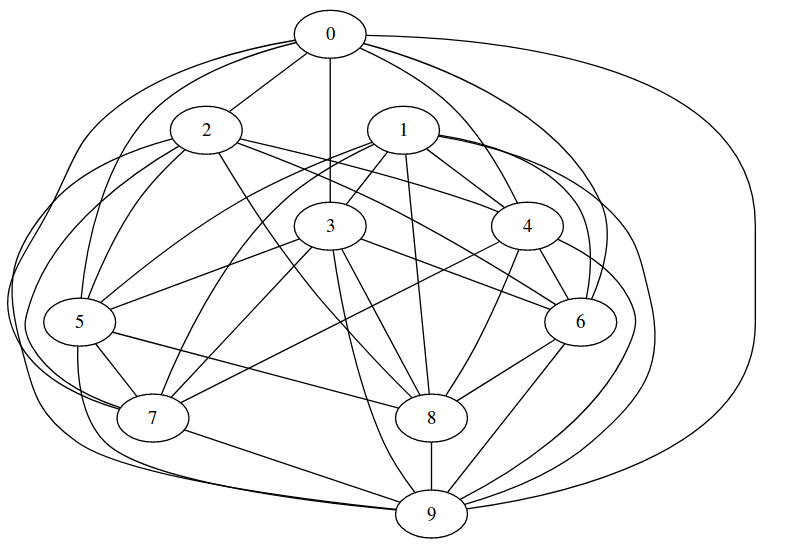
\includegraphics[scale=0.45]{10.png}

\item Добавяме независимо множество от 3 върха, разширявайки графа до 13 върхов граф, базирайки се на $extend$ алгоритъма: тоест, при параметри $extend$ $q$ $r$, намираме всички максимални $K_{q-1}$ свободни множества и построяваме всевъзможните графи, използвайки тези множества и добавените независими $r$ върха (в случая, търсим $K_5$-свободни множества и добавяме 3 върха) . Като резултат от $extend$ алгоритъма, получаваме максималните 13 върхови графи. Накрая премахваме изоморфните графи чрез $shortg$ и разглеждаме само тези, които имат свойството $G\xrightarrow{\text{v}} (2, 3, 4)$

\begin{lstlisting}[language=bash]
$ cat 10.g6 | ./extend 6 3 | nauty-shortg | ./fv 2 3 4
\end{lstlisting}

\item Понеже броя на резултантните графи е нула, то следва, че няма графи в множеството $H_v(2, 3, 4; 6; 13)$, които имат независимо множество от 3 върха. Остава да проверим, че и графите които не съдържат независимо множество от 3 върха не принадлежат на това множество. Това може да стане посредством графите-допълнениe на (3,6)-Рамзи графите (които имаме изчислени предварително от \cite{mckay}), които са графи, несъдържащи независимо множество с 3 върха и 6-клика.

\begin{lstlisting}[language=bash]
cat r36_13.g6 | ./complement | ./fv 2 3 4
\end{lstlisting}

Така заключaваме, че  $F_v(2,3,4;6)\geq14$.

\item Остава да докажем, че $F_v(2,3,4;6)\leq14$. В \cite{nenovnedialkov} е даден пример за такъв граф, който дава оценката отгоре. Може да докажем твърдението и с помощта на изчисления, използвайки отново (3,6)-Рамзи графите:

\begin{lstlisting}[language=bash]
cat r36_14.g6| ./complement | ./fv 2 3 4
\end{lstlisting}

Получаваме следните два графа (които нямат независимо множество с 3 върха и нямат 6-клика):

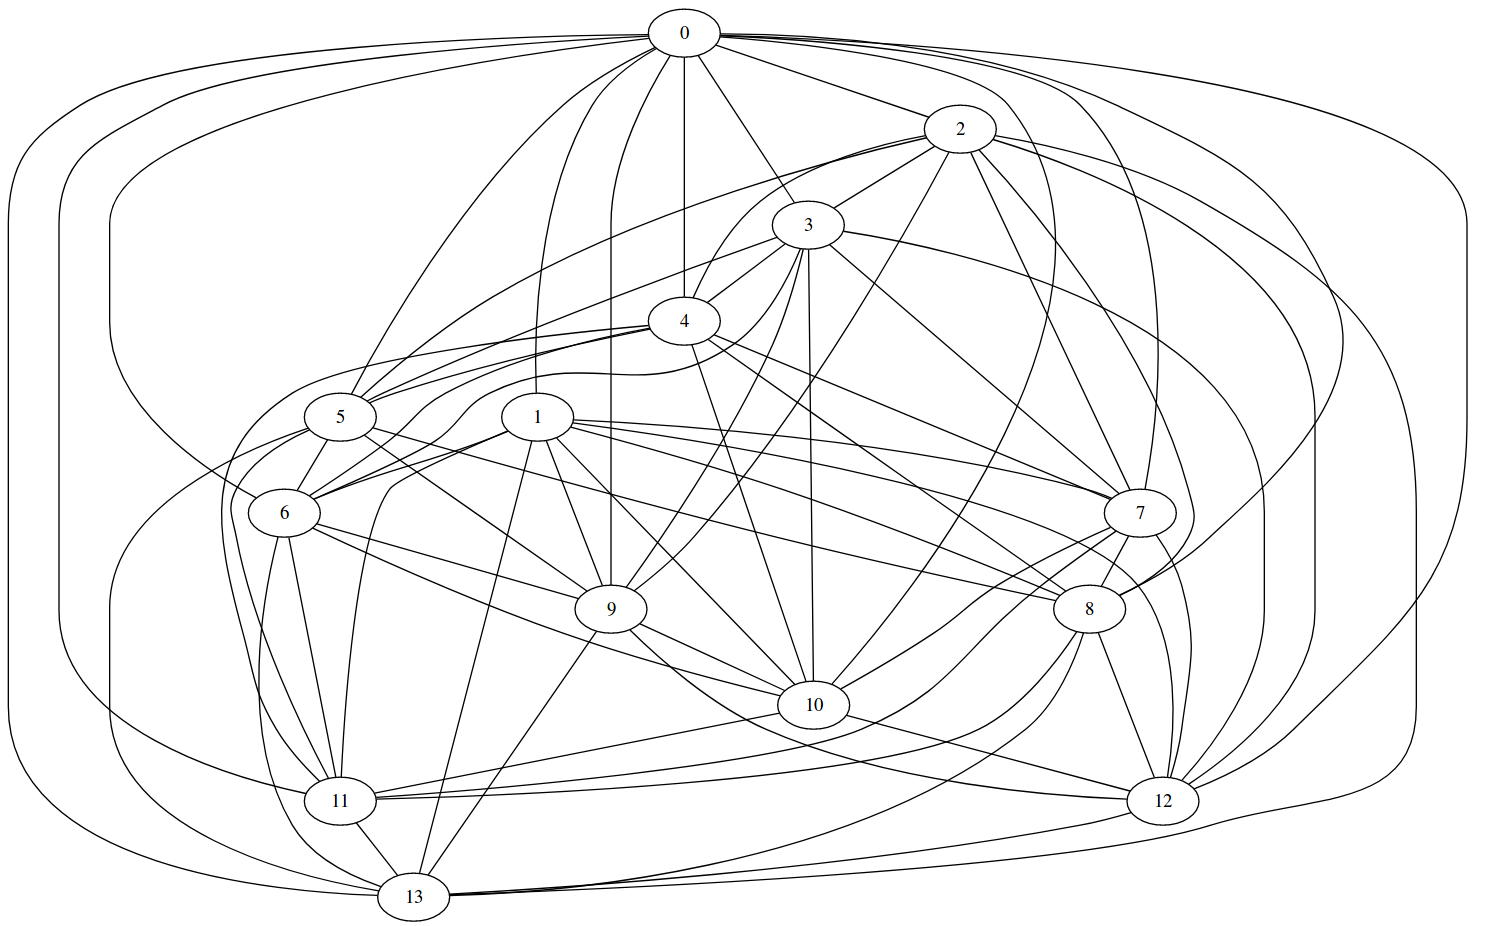
\includegraphics[scale=0.25]{first14vertex.png}

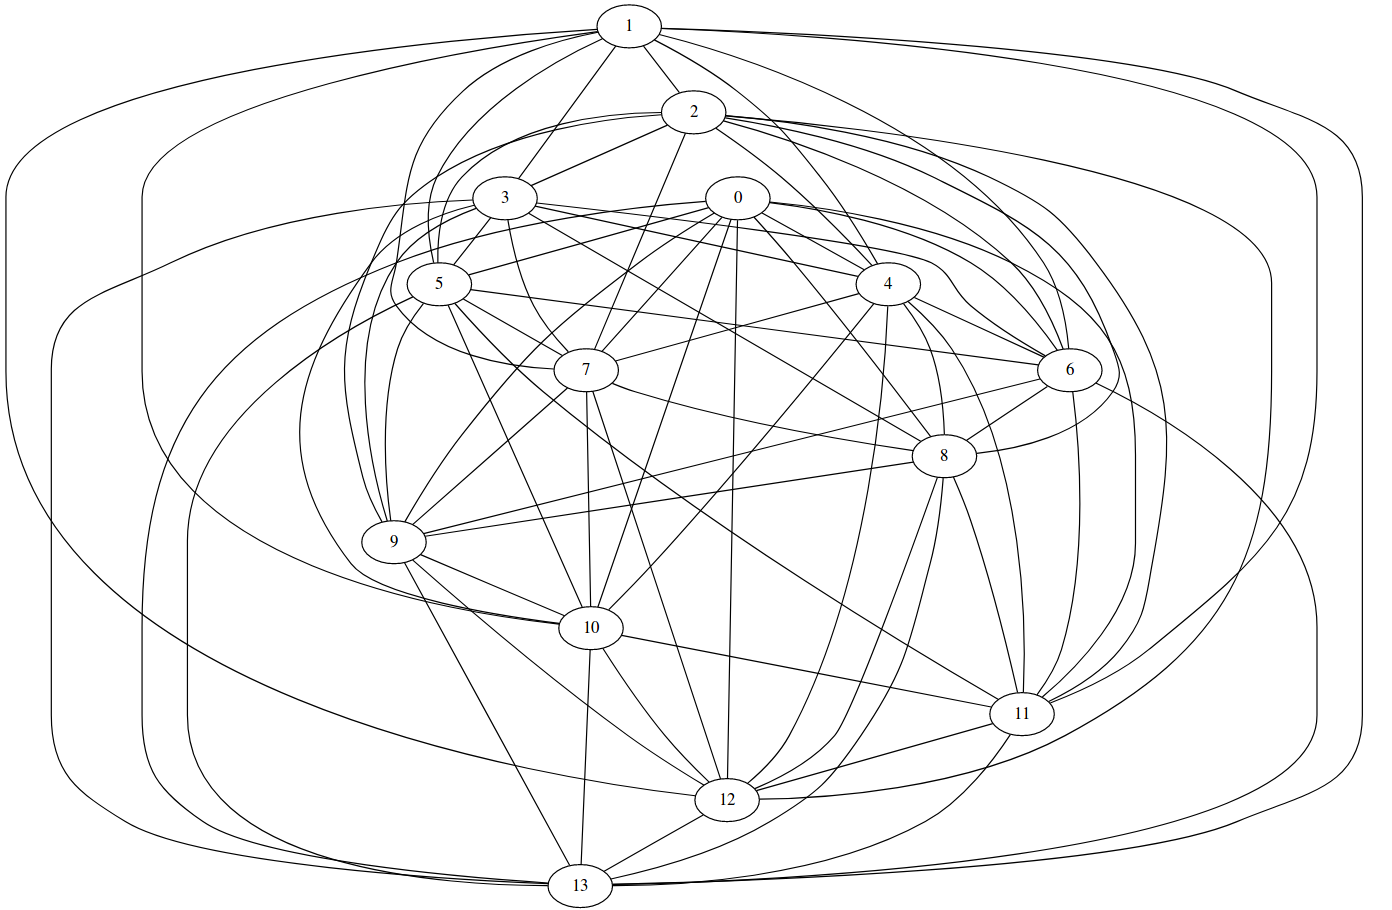
\includegraphics[scale=0.25]{second14vertex.png}

Така доказахме, че $F_v(2,3,4;6)=14$.

\end{enumerate}
 
\begin{thebibliography}{99}

\bibitem{mckay} https://users.cecs.anu.edu.au/~bdm/data/ramsey.html

\bibitem{nenovnedialkov}
Nedyalkov, Evgeni & Nenov, Nedyalko. (2002). Computation of the Vertex Folkman Numbers F(2, 2, 2, 4;6) and F(2, 3, 4;6).. Electr. J. Comb.. 9. 

\end{thebibliography}


\end{document}
